\section{Method}\label{meth}
Consider a population stratified by $N_g$ patches and $N_a$ age groups.%
\footnote{We use different notation than \citet{Arenas2020};
  a comparison is given in Table~\ref{tab:notation}.}
Let $P_{ga}$ be the number of people in patch $g$ and age group $a$.
Let $y$ denote $N_y$ different types of contacts.
Let $B_{gg'}$ be the proportion of population $P_{g}$ who travel to $g'$ each day,
or the ``mobility matrix''.%
\footnote{\citet{Arenas2020} consider different mobility patterns by age: $B_{gg'a}$.
  For simplicity, we consider $B_{gg'}$ unstratified by age,
  but age stratification could be added to our approach.}
% ==================================================================================================
\subsection{Original Approach}\label{meth.orig}
\citet{Arenas2020} model the force of infection (incidence) experienced by population $P_{ga}$ as:
\begin{equation}\label{eq:Arenas.lambda}
  \lambda_{ga}(t) = (1-\rho_a)\,\Phi_{ga}(t) + \rho_a \sum_{g^*} B_{gg^*a} \Phi_{g^*a}(t)
\end{equation}
where:
$\Phi_{ga}(t)$ is the probability of acquiring infection while in patch $g$;
and $\rho_{a} \in [0,1]$ is an age-specific overall mobility factor.
Thus, $\lambda_{ga}(t)$ is the sum of infection probabilities
from the residence patch $g$, and from visited patches $g^* \ne g$.
The probability $\Phi_{g^*a}(t)$ is modelled using
the chained binomial for multiple exposures \cite{Kaplan1990}:
\begin{equation}\label{eq:Arenas.Phi}
  \Phi_{g^*a}(t) = 1 - \prod_{a'}\prod_{g'} \prod_{i'} {\left(1 - \beta_{i'}\right)}
    ^{\,f_{g^*}C_a\,\theta_{aa'} \Omega_{g^*g'i'a'}}
\end{equation}
where:
$\beta_i$ is the per-contact transmission probability associated with infectious state $i$;
$f_{g^*}$ is a density factor associated with patch $g^*$; % (that we won't consider further here);
$C_a$ is the expected number of contacts made per person per day in age group $a$;
$\theta_{aa'}$ is the age distribution of those contacts, derived from \cite{Prem2017} for Spain,
such that $\sum_{a'} \theta_{aa'} = 1$;
and $\Omega_{g^*g'i'a'}$ is the proportion of individuals present in patch $g^*$
who reside in patch $g'$ and who are in infectious state $i'$, for each age group $a'$.
This proportion $\Omega_{g^*g'i'a'}$ is defined as:
\begin{equation}\label{eq:Arenas.Omega}
  \Omega_{g^*g'a'i'} = \frac{P_{g'i'a'} M_{g'g^*a'}}{\sum_{g'i'} P_{g'i'a'} M_{g'g^*a'}}
\end{equation}
where $M_{gg'a}$ is a convenience simplification of the mobility matrix:
\begin{equation}\label{eq:Arenas.M}
  M_{gg'a} = (1-\rho_a)\,\delta_{gg'} + \rho_a B_{gg'a}
\end{equation}
This model of infection captures important mixing patterns related to recurrent mobility
that are relevant to epidemic modelling on relatively small spatial and time scales.
However, the model could be improved by
separating different contact types throughout the force of infection equation,
and by not fixing the age distribution of contacts.
Three specific issues with the original approach are as follows.
\begin{enumerate}
  \item \textbf{Contact balancing:}\label{issue:balance}
  The contact balancing principle states that
  the total number of contacts formed by group $a$ with group $a'$
  should equal the number formed by group $a'$ with group $a$ \cite{Arregui2018}:
  \begin{equation}\label{eq:balance}
    P_{a} C_{a} \theta_{aa'} = P_{a'} C_{a'} \theta_{a'a}
  \end{equation}
  For a model with non-random age mixing but random mixing by patches,
  Eq.~(\ref{eq:balance}) could be satisfied by a single fixed age mixing matrix $\theta_{aa'}$,
  i.e. for the population overall.
  However, in the context of patch-based mixing reflecting recurrent mobility,
  Eq.~(\ref{eq:balance}) should be satisfied in each mixing context (patch).
  If different patches have different age distributions,
  then it would not be possible to satisfy Eq.~(\ref{eq:balance})
  with a single fixed age mixing matrix $\theta_{aa'}$.
  The implications of violating Eq.~(\ref{eq:balance}) depend on the context.
  For example, if $\theta_{aa'}$ overestimates
  the proportion of contacts formed with a highly infectious age group,
  then the modelled incidence would be higher than it should be, etc.
  \item \textbf{Age mixing by contact type:}\label{issue:age-mix}
  A related issue is that the expected contact rates by age group $C_a$ reflect
  the summation of different types in \cite{Arenas2020},
  and so the fixed age mixing matrix $\theta_{aa'}$ is applied to all contact types.
  Then, when restrictions are simulated, overall average contact rates $C_a$ are reduced
  by an amount reflecting the proportion of work versus home contacts
  (and various related assumptions), but $\theta_{aa'}$ is not updated.
  As illustrated by the \polymod study \cite{Mossong2008}, age mixing patterns vary by contact type.
  Thus, differential reductions in each contact type would affect age mixing patterns.
  For example, if reduced contacts between working-aged adults were not reflected in $\theta_{aa'}$,
  then the relative contribution of this age group to transmission could be overestimated.
  \item \textbf{Modelling contact \& mobility reductions:}\label{issue:mobility}
  The term $(1-\rho_a)\,\Phi_{ga}(t)$ in Eq.~(\ref{eq:Arenas.lambda})
  represents transmission to non-mobile individuals in patch $g$.  
  The associated definitions in Eqs.~(\ref{eq:Arenas.Phi}--\ref{eq:Arenas.M})
  consider transmission to these individuals from visitors to patch $g$.
  Such definitions therefore imply that
  non-mobile individuals still form contacts with visitors to their residence patch.
  However, when simulating confinement measures in \cite{Arenas2020},
  mobility reductions are always paired with proportional reductions in non-home contacts,
  suggesting that non-mobile individuals form only home contacts.
  It seems incongruous to model the formation of
  home contacts among non-mobile residents of patch $g$ with mobile visitors to patch $g$.
  As illustrated in Figure~\ref{fig:nm}, this approach potentially
  overestimates the contact network connectivity during reduced mobility
  versus an approach in which non-mobile populations do not contact visitors,
  and thus could underestimate the impact of confinement strategies.
  While it may be sometimes desirable to allow mixing of ``non-mobile'' individuals
  with visitors to their residence patch,
  the original approach does not provide parameterization to prevent this from happening.
  % The differences in connectivity between the approaches are larger when
  % mobility reductions differ by patch.
\end{enumerate}
We therefore develop a refinement of the original approach,
with the aim of addressing these three issues.
% ==================================================================================================
\subsection{Proposed Approach}\label{meth.prop}
In the proposed approach, the contributions of different contact types to the force of infection
are added to the binomial function for multiple exposures:
\begin{equation}
  \lambda_{ga}(t) = 1 - \prod_{y}\prod_{g'}\prod_{a'}\prod_{i'} {\left(1 - \beta_{i'}\right)}
  ^{C_{gag'a'y} \Omega_{g'a'i'}}
\end{equation}
where:
$C_{gag'a'y}$ is the expected number of type $y$ contacts formed per person per day
among individuals in population $P_{ga}$ with those in population $P_{g'a'}$;
and $\Omega_{g'a'i'}$ is the proportion of individuals in residing in patch $g'$ and age group $a'$
who are in infectious state $i'$:
\begin{equation}
  \Omega_{g'a'i'} = \frac{P_{g'a'i'}}{P_{g'a'}}
\end{equation}
For each type of contact, $C_{gag'a'y}$ is defined to reflect
both age-related and mobility-related mixing factors,
as described in the following subsections.
To support these descriptions, we will refer to Figures from an example application,
although the details of the application and the Figures are given in \S~\ref{ex}.
Collecting the full network of contacts in the matrix $C_{gag'a'y}$ is parsimonious,
and allows us to easily compute various properties, like the margins in $a,a'$ or $g,g'$,
and whether contact balancing is satisfied per Eq.~(\ref{eq:balance}).
Additionally, separating contact types allows the incorporation of
different probabilities of transmission per contact type $\beta_{i'y}$, if desired.
% --------------------------------------------------------------------------------------------------
\subsubsection{Age Mixing}\label{meth.prop.mix.age}
\citet{Prem2017} project contact patterns by 5-year age groups
from the \polymod study \cite{Mossong2008} onto 152 countries,
considering various demographic data.
These contact matrices represent $C_{aa'y}$:
the expected number of type $y$ contacts formed per day among
individuals in age group $a$ with those in age group $a'$.
Four types of contact are considered: ``home'', ``work'', ``school'', and ``others''%
\footnote{The ``others'' contact type in \cite{Prem2017} is itself derived from
  the combination of ``leisure'', ``transport'', and ``other'' contact types from \cite{Mossong2008},
  while the ``home'', ``work'', and ``school'' types are the same between the studies.}
(Figure~\ref{fig:C4AAy0}).
We aim to incorporate these contact numbers and patterns into $C_{gag'a'y}$.
\par
The first challenge is that these contact matrices $C_{aa'y}$ are
inherently weighted by the underlying population age distribution---%
the proportion of expected contacts with age group~$a'$ is proportional to the size of age group~$a'$.
To overcome this challenge and apply these patterns to new population age structures, 
\citet{Arregui2018} suggest to divide by the population age distribution
to obtain an ``unweighted'' matrix $C^u_{aa'y}$ (Figure~\ref{fig:C4AAy1}):%
\footnote{The matrix $C^u_{aa'y}$ could also be interpreted as
  the expected contact matrix for a population with a rectangular demographic pyramid \cite{Arregui2018}.}
\begin{equation}\label{eq:C^u}
  C^u_{aa'y} = C_{aa'y} \frac{\bar{P}}{P_{a'}}
\end{equation}
where $\bar{P}$ is the mean of $P_{a'}$.
\par
The next challenge is that $C^u_{aa'y}$ may not satisfy
the contact balancing principle, Eq.~(\ref{eq:balance}),
due to potential differences in age distribution of
the \polymod survey respondents versus that of the contacts the respondents reported.
In order to ensure that $C_{gag'a'y}$ will satisfy the balancing principle,
$C^u_{aa'y}$ must satisfy the principle.
A simple solution is to average $C^u_{aa'y}$ with its transpose
to obtain the ``balanced'' matrix $C^{ub}_{aa'y}$ (Figure~\ref{fig:C4AAy2}):
\begin{equation}\label{eq:C^ub}
  C^{ub}_{aa'y} = \frac{1}{2}\left[C^u_{aa'y} + {C^u_{aa'y}}^{T}\right]
\end{equation}
This operation may change the margin $C_{ay}$, representing
the total type $y$ contacts formed by individuals in age group $a$.
However, such changes are reasonable if understood as a correction for sampling bias.%
\footnote{A perfect survey in a closed population would produce
  a contact matrix $C^u_{aa'y}$ that is already balanced.}
\par
A final challenge in applying the contact matrices from \cite{Prem2017} is that
the 5-year age groups may not align with the age groups of interest.
Overcoming this challenge is not theoretically required to obtain $C_{gag'a'y}$,
but we describe a solution here in case it is useful for modelling applications.
We begin by upsampling the contact matrix from 5-year age groups $a_5$ to 1-year age groups $a_1$
using bilinear interpolation, based on the midpoints of each age group,
and scaled by a factor of $1/5$.
To avoid edge effects associated with many interpolation implementations,
we first pad the matrix by replicating the edges diagonally.
If the desired age groups extend beyond the maximum age group of 80 available in \cite{Arenas2020},
diagonal padding can also be used to approximate the trends in the additional age groups.
Then, given the age groups of interest $a_*$ (which may have irregular widths),
we aggregate $C^{ub}_{a_1a'_1y}$ to obtain $C^{ub}_{a_*a'_*y}$
using matrix multiplication with indicator matrix $A$:
\begin{equation}\label{eq:Ca*}
  C^{ub}_{a_*a'_*y} = \frac{A_{a_*a_1}}{\sum_{a_1} A_{a_*a_1}} C^{ub}_{a_1a'_1y} A_{a'_*a'_1}^T,\qquad
  A_{a_*a_1} = \begin{cases}
    1, & a_1 \in a_* \\
    0, & a_1 \not\in a_* \\
  \end{cases}
\end{equation}
The right-hand $A^T$ term \textit{sums} the total number of contacts
formed with the 1-year ``other'' age groups $a'_1$ corresponding to $a'_*$.
The left-hand $A$ term \textit{averages} the total number of contacts
formed from the 1-year ``self'' age groups $a_1$ corresponding to $a_*$.
The average weights each 1-year age group $a_1$ equally,
although other weights could be incorporated through the nonzero values of $A$.
Another interpretation of the normalization sum is the widths of the age groups $a_*$.
\par
The resulting matrix $C^{ub}_{a_*a'_*y}$ represents the expected contacts among age groups $a_*$
when mixing with a population having equal proportion in all age groups $a'_*$ (regardless of their width).
Thus, $C^{ub}_{a_*a'_*y}$ can later be multiplied by the population age distribution of interest%
---reversing Equation~(\ref{eq:C^u})---%
to obtain the expected number of contacts when mixing with that population.
This approach then addresses issues \ref{issue:balance}~and~\ref{issue:age-mix}
described in \S~\ref{meth.orig}.
% --------------------------------------------------------------------------------------------------
\subsubsection{Mobility-Related Mixing}\label{meth.prop.mix.mob}
For mobility-related mixing, we use the same mobility matrix $B_{gg'}$ as \cite{Arenas2020},
representing the expected proportions of individuals in patch $g$ who travel to patch $g'$ each day.
We do not assume that rows of $B_{gg'}$ sum to~1;
however, we do assume that the diagonal ($g=g'$) represents
the proportion of individuals who are mobile within their own patch.
Thus $1 - \sum_{g'} B_{gg'}$ represents
the proportion of individuals in patch $g'$ who are not mobile.
In \S~\ref{app.mob} we discuss some details about generating such a matrix $B_{gg'}$.
\par
The distinction between ``not mobile'' and ``mobile within the residence patch''
is new versus the original approach \cite{Arenas2020}.
As described in \S~\ref{meth.orig}, in the original approach,
individuals with reduced mobility were assumed to form fewer contacts,
but continue mixing with visitors to their residence patch.
Our proposed distinction allows us to separate two ``mixing pools'' where contacts might be formed:
``home pools'', where contacts are formed exclusively with
other residents of the same patch $g$ (e.g. household contacts); and
``travel pools'', where contacts are formed with any mobile individuals visiting patch $g$,
which may include individuals who are mobile within their residence patch
and travellers from other patches (e.g. work contacts).
An illustration of these pools is given in Figure~\ref{fig:pools}.
\begin{figure}
  \centering
  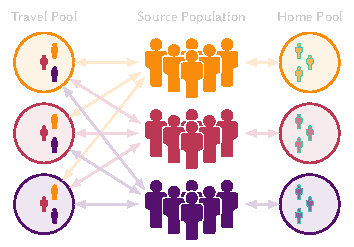
\includegraphics[width=.6\linewidth]{pools-half-home}
  \caption{Toy example of ``home'' vs ``travel'' mixing pools
    for a network with 3 patches and 50\% individuals mobile.
    Contacts in the home pool are formed exclusively with other members of the residence patch,
    whereas contacts in the travel pool may be formed with any visitors to the patch}
  \label{fig:pools}
  \floatfoot{Non-mobile populations are indicated with faded colour and green outline}
\end{figure}
\par
We assume that individuals who are not mobile will only form contacts within the home pool,
but that the number of contacts formed per person within the home pool is fixed and not affected by
the proportion of individuals who are not mobile.
It is not necessary to assume that
all contacts of any particular type are formed with only one type of pool;
rather we introduce a parameter $h_y \in [0,1]$ representing
the proportion of type $y$ contacts that are formed with the home pool.
For example, we could have
$h_y = 1$ for household contacts, $h_y = 0$ for work contacts, and perhaps $h_y = 0.5$ for school contacts.
\par
To calculate $C_{gag'a'y}$ using these assumptions, we begin by considering the travel pool in patch $g^*$.
The effective number of individuals from population $P_{ga}$
who are present in the pool is given by:%
\footnote{If residents of different patches might have relatively different numbers of contacts,
  a scaling factor could be applied here.}
\begin{equation}\label{eq:P*}
  P^{\,g^*}_{gay} = h_y P_{ga} B_{gg^*}
\end{equation}
If we assume that mixing by residence patch $g$ within the pool is random,
we need only consider age mixing within the pool.
Under completely random mixing,
the total number of contacts formed between $P^{\,g^*}_{gay}$ and $P^{\,g^*}_{g'a'y}$
is given by the outer product:
\begin{equation}\label{eq:X*r.gagay}
  X^{g^*r}_{gag'a'y} = P^{\,g^*}_{gay} \otimes \left. P^{\,g^*}_{g'a'y} \middle/ \textstyle\sum_{g'a'} P^{\,g^*}_{g'a'y}\right.
\end{equation}
where the first term represents the absolute population size of ``self'',
and the second term represents proportions of their contacts among ``other'' strata.
Then, the patterns of age mixing can be applied via multiplication:
\begin{equation}\label{eq:X*.gagay}
  X^{g^*}_{gag'a'y} = X^{g^*r}_{gag'a'y} \left.C^{ub}_{aa'y} \middle/ \textstyle\sum_{a'_1} A_{a'a'_1}\right.
\end{equation}
since $X^{g^*r}_{gag'a'y}$ is proportional to the population age distribution of ``others'',
and will therefore act to reverse Eq.~(\ref{eq:C^u}) as planned.
The term $\sum_{a'_1} A_{a'a'_1}$ is from Eq.~(\ref{eq:Ca*}),
representing the widths of the age groups $a'$.
It is necessary to divide by the widths of age groups $a'$ since
both $X^{g^*r}_{gag'a'y}$ and $C^{ub}_{aa'y}$ are proportional to these widths,
but the proportionality should only be singular overall.
We could have applied this normalization to $C^{ub}_{aa'y}$
in Eq.~(\ref{eq:Ca*}) in the same way as for $a$,
but this would make $C^{ub}_{aa'y}$ harder to interpret,
as it would no longer represent the expected numbers of contacts for each age group.
\par
Mixing within home pools can be modelled similar to mixing within travel pools,
with one small modification: replacing $B_{gg'}$ with the identity matrix $\delta_{gg'}$.
Following through Eqs.~(\ref{eq:P*}--\ref{eq:X*r.gagay}), we obtain $X^{h}_{gag'a'y}$,
representing the total contacts formed within home pools.
Then, the total type $y$ contacts formed between populations $P_{ga}$ and $P_{g'a'}$
across all relevant mixing pools is given by the sum:
\begin{equation}\label{eq:Xgagay}
  X_{gag'a'y} = X^h_{gag'a'y} + \sum_{g^*} X^{g^*}_{gag'a'y}
\end{equation}
It may be tempting to simplify the model for home pool contacts by
updating the mobility matrix $B_{gg'}$ similar to Eq.~(\ref{eq:Arenas.M}), with $h_y = (1-\rho_a)$.
However, such an approach does not produce the same result as Eq.~(\ref{eq:Xgagay}),
and indeed underpins issue \ref{issue:mobility} described in \S~\ref{meth.orig}
regarding mixing of non-mobile individuals with mobile visitors to their patch.
On the other hand, if the interpretation of ``non-mobile'' is intended to allow mixing with visitors,
then $B_{gg'}$ can still be adjusted per Eq.~(\ref{eq:Arenas.M}) to simulate this behaviour.
Another implication of our approach is that
non-mobile individuals will not form mobility-related contacts;
thus if $\sum_{g'} B_{gg'}$ is reduced,
the total contacts formed by residents of patch $g$ would be reduced proportionately.
\par
Finally, the number of type $y$ contacts formed \textit{per person}
in population $P_{ga}$ with population $P_{g'a'}$ can be obtained by
dividing $X_{gag'a'y}$ by the population size:
\begin{equation}\label{eq:Cgagay}
  C_{gag'a'y} = \frac{X_{gag'a'y}}{P_{ga}}
\end{equation}